

\emph{Vaadin}~\cite{vaadin} es un \textbf{framework} para el desarrollo de aplicaciones \emph{web} avanzadas, también conocidas como \emph{Rich-Internet Applications (RIA)}~\cite{ria}. El objetivo del paradigma \emph{RIA} es desarrollar aplicaciones \emph{web} con interfaces avanzadas que les haga asemejarse a las aplicaciones de escritorio. La principal ventaja que aporta \emph{Vaadin} es que permite escribir aplicaciones en código Java, como si fuesen de escritorio, y luego este código es transformado para que funcione en tecnologías web como HTML (HyperText Markup Language)~\cite{html}, CSS (Cascading Style Sheets)~\cite{css}, Javascript~\cite{javascript}, HTTP (Hypertext Transfer Protocol)~\cite{http} o AJAX (Asynchronous JavaScript and XML)~\cite{ajax}.

Una de las características diferenciadores de \texttt{Vaadin} es que, al contrario de las librerías de JavaScript tradicionales, \emph{Vaadin} también contempla la parte del servidor, por lo se generan tanto las llamadas al servidor desde la interfaz gráfica (\emph{front-end}) como la recepción y tratamiento de esas llamadas en la parte del servidor (\emph{back-end}).



 	
 \subsection{Ejemplo Vaadin}
 	
\begin{figure}[!tb]
	\centering
	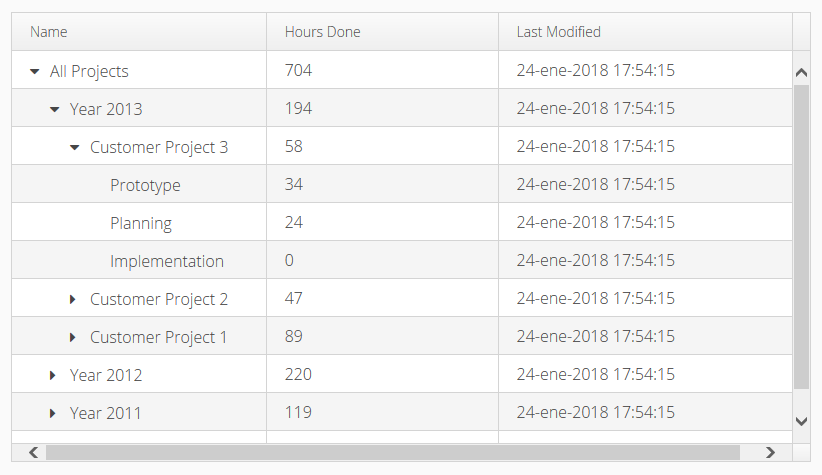
\includegraphics[width=\linewidth]{vaadinExampleImage.png}
	\caption{Árbol de Proyectos}
	\label{fig:vaadinExampleImage}
\end{figure}

A continuación, se explica un ejemplo de contrucción de una jerarquía de tareas propias en la gestión de proyectos por parte de un Jefe de Proyecto (Figura~\ref{fig:vaadinExampleImage}).

El proyecto creado para realizar el ejemplo se compone de una interfaz de usuario (Figura~\ref{fig:uiVaadin}) la cuál utiliza un componente llamado TreeGrid  (será explicado posteriormente,Figura~\ref{fig:treeGrid}) y un contenedor de datos (Figura~\ref{fig:demoContainer}).

Para entrar en contexto con la implementación de un proyecto en Vaadin, es necesario recalcar que el objetivo es abstraer al usuario de todo el comportamiento gráfinco implementado en HTML o Javascript, por lo tanto, para poder crear las estructuras que finalmente desembocarán en elementos gráficos, Vaadin utiliza los llamados componentes.

Un componente es una interfaz de alto nivel, todo elemento gráfico que se quiera utilizar debe de implementar y extender de las clases \emph{Component}\cite{componentVaadin} y \emph{AbstractComponent}\cite{abstractComponentVaadin}, éstas constan de toda la implementación por defecto necesaria para poder mostrar un elemento.

La Figura~\ref{fig:uiVaadin} reprensenta la interfaz gráfica que se ha implementado para el ejemplo. En ella podemos ver que se ha creado un \emph{layout} o espacio reservado en la interfaz para insertar componentes, y se le ha establecido dos características, la primera es un espaciado entre los componentes y la segunda es un márgen sobre los cuatro lados del componente (Figura~\ref{fig:uiVaadin}, Líneas~4-6).

Posteriormente se declara el componente \emph{TreeGrid} que será el encargado de representar la jerarquía de elementos, además, se le ha dado un ancho y alto al elemento de 800 y 450 píxeles respectivamente (Figura~\ref{fig:uiVaadin}, Líneas~8-10).

Para que un componente muestre datos se le debe de insertar un contenedor de datos, en nuestro caso se ha creado una clase que se explicará más adelante que proporciona esta característica, y se le insertado a dicho componente (Figura~\ref{fig:uiVaadin}, Líneas~12-13).

Por último, se ha añadido el componente al \emph{layout} y este al contenido de la interfaz (Figura~\ref{fig:uiVaadin}, Líneas~15-16).

\begin{figure}[!tb]
	\centering
	\begin{lstlisting}[language=Java]
	@Override
	protected void init(VaadinRequest request) {
	
		final VerticalLayout layout = new VerticalLayout();
		layout.setSpacing(true);
		layout.setMargin(true);
		
		final TreeGrid grid = new TreeGrid();
		grid.setWidth(800, Unit.PIXELS);
		grid.setHeight(450, Unit.PIXELS);
		
		DemoContainer container = new DemoContainer();
		grid.setContainerDataSource(container);
		
		layout.addComponent(grid);
		setContent(layout);
	}\end{lstlisting}
	\caption{Interfaz de Usuario Vaadin}
	\label{fig:uiVaadin}
\end{figure}

La clase \emph{TreeGrid} es la encargada de mostrar los datos de forma jerárquica. Para cumplimentar esta interfaz, se extiende de la clase de Vaadin \emph{Grid} la cuál permite crear una tabla de forma sencilla con solo implemetar sus métodos. Respecto a la clase \emph{TreeGrid}, con extenderla, ya es capaz de crear una lista jerárquica sobre la tabla. Esta clase posee métodos para añadir y eliminar \emph{listeners} para contraer y expandir el árbol de elementos (Figura~\ref{fig:treeGrid}, Líneas~18-32), para \emph{settear} (Figura~\ref{fig:treeGrid}, Líneas~3-15), y el método para ver desde fuera el estado del componente (Figura~\ref{fig:treeGrid}, Líneas~35-38). El estado del \emph{TreeGrid} es una clase que contiene el identificador de la columna que está siendo modificada por el usuario (Figura~\ref{fig:treeGridState}).


\begin{figure}[!tb]
	\centering
	\begin{lstlisting}[language=Java]
	public class TreeGrid extends Grid {
		
		@Override
		public void setContainerDataSource(Container.Indexed container) {
			if (container != null) {
				if (!(container instanceof Container.Hierarchical)) {
					container = new IndexedContainerHierarchicalWrapper(container);
				}
				
				if (!(container instanceof Collapsible)) {
					container = new ContainerCollapsibleWrapper(container);
				}
			}
			super.setContainerDataSource(container);
		}
		
		
		public void addExpandListener(ExpandEvent.ExpandListener listener) {
			addListener(ExpandEvent.class, listener, ExpandEvent.ExpandListener.EXPAND_METHOD);
		}
		
		public void removeExpandListener(ExpandEvent.ExpandListener listener) {
			removeListener(ExpandEvent.class, listener, ExpandEvent.ExpandListener.EXPAND_METHOD);
		}
		
		public void addCollapseListener(CollapseEvent.CollapseListener listener) {
			addListener(CollapseEvent.class, listener, CollapseEvent.CollapseListener.COLLAPSE_METHOD);
		}
		
		public void removeCollapseListener(CollapseEvent.CollapseListener listener) {
			removeListener(CollapseEvent.class, listener, CollapseEvent.CollapseListener.COLLAPSE_METHOD);
		}
		
		
		@Override
		protected TreeGridState getState() {
			return (TreeGridState) super.getState();
		}
	}\end{lstlisting}
	\caption{Componente TreeGrid}
	\label{fig:treeGrid}
\end{figure}

\begin{figure}[!tb]
	\centering
	\begin{lstlisting}[language=Java]
	public class TreeGridState extends GridState {
		public String hierarchyColumnId;
	}\end{lstlisting}
	\caption{Componente TreeGrid}
	\label{fig:treeGridState}
\end{figure}


La última clase para explicar es \emph{DemoContainer}  (Figura~\ref{fig:demoContainer}), esta clase extiende de una clase de Vaadin llamada \emph{HierarchicalContainer} que se encarga de realizar toda la lógica para expandir y contraer los nodos, además, implementa las clases de Vaadin \emph{Collapsible} (Figura~\ref{fig:demoContainerCollapsible}) y \emph{Measurable} (Figura~\ref{fig:demoContainerMeasurable}), encargadas de colapsar el árbol de elementos y de calcular la profundidad del elemento en la jerarquía respectivamente.




\begin{figure}[!tb]
	\centering
	\begin{lstlisting}[language=Java]
	public class DemoContainer extends HierarchicalContainer implements Collapsible, Measurable {
	
		static final String PROPERTY_NAME = "Name";
		static final String PROPERTY_HOURS = "Hours done";
		static final String PROPERTY_MODIFIED = "Last modified";
		
		public DemoContainer() {
			addContainerProperty(PROPERTY_NAME, String.class, "");
			addContainerProperty(PROPERTY_HOURS, Integer.class, 0);
			addContainerProperty(PROPERTY_MODIFIED, Date.class, new Date());
			
			for (Object[] r : DataSource.getRoot()) {
				addItem(r);
			}
			
			setItemSorter(new DemoItemSorter());
		}
		
		private Object addItem(Object[] values) {
			Item item = addItem((Object) values);
			setProperties(item, values);
			return values;
		}
		
		private Object addChild(Object[] values, Object parentId) {
			Item item = addItemAfter(parentId, values);
			setProperties(item, values);
			setParent(values, parentId);
			return values;
		}
		
		private void setProperties(Item item, Object[] values) {
			item.getItemProperty(PROPERTY_NAME).setValue(values[0]);
			item.getItemProperty(PROPERTY_HOURS).setValue(values[1]);
			item.getItemProperty(PROPERTY_MODIFIED).setValue(values[2]);
		}

		private void addChildren(Object itemId) {
			for (Object[] child : DataSource.getChildren(itemId)) {
				Object childId = addChild(child, itemId);
				if (Boolean.TRUE.equals(expandedNodes.get(childId))) {
					addChildren(childId);
				}
			}
		}
		
		private boolean removeChildrenRecursively(Object itemId) {
			boolean success = true;
			Collection<?> children2 = getChildren(itemId);
			if (children2 != null) {
				Object[] array = children2.toArray();
				for (int i = 0; i < array.length; i++) {
					boolean removeItemRecursively = removeItemRecursively(
					this, array[i]);
					if (!removeItemRecursively) {
						success = false;
					}
				}
			}
			return success;	
		}
		
		@Override
		public boolean hasChildren(Object itemId) {
			return !DataSource.isLeaf(itemId);
		}
		
	}\end{lstlisting}
	\caption{Contenedor TreeGrid}
	\label{fig:demoContainer}
\end{figure}


\begin{figure}[!tb]
	\centering
	\begin{lstlisting}[language=Java]
	public class DemoContainer
	
		...
	
		private Map<Object, Boolean> expandedNodes = new HashMap<>();
			
		@Override
		public void setCollapsed(Object itemId, boolean collapsed) {
			expandedNodes.put(itemId, !collapsed);	
			if (collapsed) {
				removeChildrenRecursively(itemId);
			} else {
				addChildren(itemId);
			}
		}
		
		@Override
		public boolean isCollapsed(Object itemId) {
			return !Boolean.TRUE.equals(expandedNodes.get(itemId));
		}
	}\end{lstlisting}
	\caption{Contenedor TreeGrid Collapsible}
	\label{fig:demoContainerCollapsible}
\end{figure}

\begin{figure}[!tb]
	\centering
	\begin{lstlisting}[language=Java]	
	public class DemoContainer
	
		...
		@Override
		public int getDepth(Object itemId) {
			int depth = 0;
			while (!isRoot(itemId)) {
				depth ++;
				itemId = getParent(itemId);
			}
			return depth;
		}
	}\end{lstlisting}
	\caption{Contenedor TreeGrid Measurable}
	\label{fig:demoContainerMeasurable}
\end{figure}


Con estas indicaciones se ha creado un ejemplo sencillo de composición de elementos jerárquicos entre sí utilizando Vaadin, como podemos ver ha facilitado mucho su implementación respecto a una configuración basada en \emph{HTML} o \emph{Javascript}.

